\documentclass[12pt,a4paper,twoside,openright]{report}
	\usepackage[hyphens,spaces,obeyspaces]{url}
	\usepackage[pdfborder={0 0 0}]{hyperref}    % turns references into hyperlinks
	\usepackage[margin=25mm]{geometry}  % adjusts page layout
	\usepackage{graphicx}  % allows inclusion of PDF, PNG and JPG images
	\usepackage{verbatim}
	\usepackage{docmute}   % only needed to allow inclusion of proposal.tex
	\usepackage{import} %import proposal from another folder
	\usepackage{pdfpages}
	\usepackage{listings}
	\usepackage{upquote}
	\usepackage{nameref}
	\usepackage{tikz}
	\usepackage{color}
	\usepackage[framemethod=tikz]{mdframed}
	\usepackage{courier}
	\usepackage{caption}
	\usepackage{subcaption}

	\definecolor{lightlightgray}{gray}{0.6}
	\definecolor{darkgreen}{rgb}{0,0.6,0}
	\definecolor{airforceblue}{rgb}{0.36, 0.54, 0.70}


	\usetikzlibrary{positioning}

	\lstset{
	language=[Objective]Caml,
	showstringspaces=false,
	breaklines=true,
	basicstyle=\normalsize\ttfamily,                 % Code font, Examples: \footnotesize, \ttfamily
	keywordstyle=\color{darkgreen},
	commentstyle=\color{airforceblue}             % Comments font
	}

	\surroundwithmdframed[
	innerleftmargin=8pt,
	innertopmargin=0pt,
	innerbottommargin=0pt]{lstlisting}

	\raggedbottom                           % try to avoid widows and orphans
	\sloppy
	\clubpenalty1000%
	\widowpenalty1000%
	
	\renewcommand{\baselinestretch}{1.1}    % adjust line spacing to make
																					% more readable
	
	\begin{document}
	
	
	%%%%%%%%%%%%%%%%%%%%%%%%%%%%%%%%%%%%%%%%%%%%%%%%%%%%%%%%%%%%%%%%%%%%%%%%
	% Title
	
	
	\pagestyle{empty}
	
	\rightline{\LARGE \textbf{Charlie Crisp}}
	
	\vspace*{60mm}
	\begin{center}
	\Huge
	\textbf{Building a Blockchain Library for OCaml} \\[5mm]
	Computer Science Tripos -- Part II \\[5mm]
	Pembroke College \\[5mm]
	\today  % today's date
	\end{center}
	
	%%%%%%%%%%%%%%%%%%%%%%%%%%%%%%%%%%%%%%%%%%%%%%%%%%%%%%%%%%%%%%%%%%%%%%%%%%%%%%
	% Proforma, table of contents and list of figures
	
	\pagestyle{plain}
	
	\chapter*{Proforma}
	
	{\large
	\begin{tabular}{ll}
	Name:               & \bf Charlie Crisp                       \\
	College:            & \bf Pembroke College                     \\
	Project Title:      & \bf Building a Blockchain Library for OCaml \\
	Examination:        & \bf Computer Science Tripos -- Part II, July 2018  \\
	Word Count:         & \bf ????\footnotemark[1]\\
	Project Originator: & KC Sivaramakrishnan                    \\
	Supervisor:         & KC Sivaramakrishnan                    
	\end{tabular}
	}
	\stepcounter{footnote}
	
	
	\section*{Original Aims of the Project}
	
	To build a library in OCaml, which can be used as a building block for Blockchain applications. 
	The library should allow participating nodes to own a shared copy of a Blockchain data structure, agreed upon using consensus.
	Nodes should also be able to commit transactions to the blockchain, which should then be visible to other participating nodes. 
	
	
	\section*{Work Completed}
	
	All that has been completed appears in this dissertation.
	
	\section*{Special Difficulties}
	
	None
	 
	\newpage
	\section*{Declaration}
	
	I, Charlie Crisp of Pembroke College, being a candidate for Part II of the Computer
	Science Tripos, hereby declare that this dissertation and the work described in it are my own work,
	unaided except as may be specified below, and that the dissertation
	does not contain material that has already been used to any substantial
	extent for a comparable purpose.
	
	\bigskip
	\leftline{Signed}
	\bigskip
	\leftline{Date}
	
	\tableofcontents
	
	\listoffigures
	
	\newpage
	\section*{Acknowledgements}
	
	I would like to thank KC Sivaramakrishnan for being an extremely helpful supervisor throughout the duration of the dissertation, as well as over the past three years.\\
	I would also like to thank Anil Madhavapeddy for allowing me to use his laptop for the duration of the dissertation, and being a very supportive DoS.\\
	Finally I'd like to thank my friends and family for supporting me through my final year.
	
	%%%%%%%%%%%%%%%%%%%%%%%%%%%%%%%%%%%%%%%%%%%%%%%%%%%%%%%%%%%%%%%%%%%%%%%
	% now for the chapters
	
	\pagestyle{headings}
	
	\chapter{Introduction}
	Blockchain technology has existed for a long time, but the definition of 'blockchain' has changed drastically since its conception.
	Previously used just to describe a data structure, the term 'blockchain' is now widely used to also describe the accompanying consensus mechanisms.
	This is mainly due to the increasing popularity of cryptocurrencies such as Bitcoin \cite{Bitcoin} which use the 'Proof of Work' algorithm to solve the double spending problem.
	Blockchain is undoubtedly the most important technology in the field of cryptocurrencies, where no single client can be trusted, however, it also has many use cases outside this sector.
	For instance, it can be used in situations where clients \textit{can} be trusted like a hospital maintaining internal medical records, or a bank wishing to record transactions from many of its own distributed clients.\\
	
	I have implemented a blockchain library in OCaml which allows the easy creation of blockchain applications.
	The blockchain is synchronised via a leader-based consensus mechanism with strict consistency.
	Developers using this library are also able to define custom validation of transactions being added to the blockchain.
	Because the application is written in OCaml, it can be compiled to bytecode, unikernels or even javascript and is therefore suitable for a wide range of destination applications and devices.

	\section{The History of the Blockchain}
	The blockchain, in its simplest form, is a series of blocks of data, where each block contains the hash of the content of the previous block. 
	Figure \ref{fig:mainblockchain} is a graphical representation of a typical blockchain data structure.\\

	\begin{figure}
		\begin{center}
			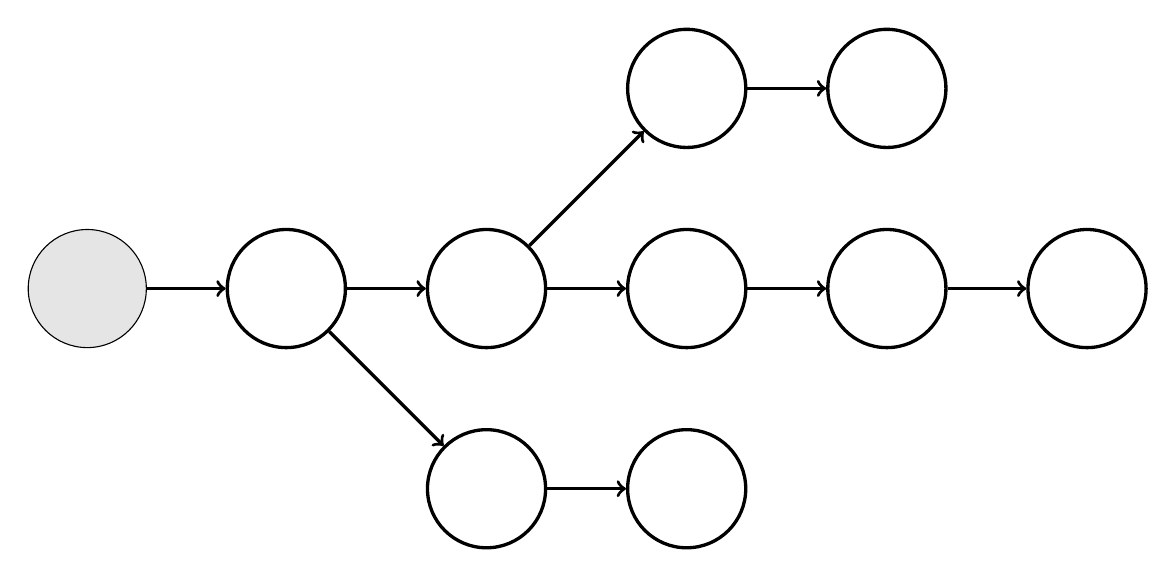
\begin{tikzpicture}[
				block/.style={circle, draw=black!100, very thick, minimum size=1.5cm},
				invis/.style={circle, draw=black!100, fill=black!10, minimum size=1.5cm}
			]
			\node[invis] (genesisblock) {};
			\node[block] (block1) [right=of genesisblock] {};
			\node[block] (block2) [right=of block1] {};
			\node[block] (block3) [right=of block2] {};
			\node[block] (block4) [right=of block3] {};
			\node[block] (block5) [right=of block4] {};
			\node[block] (sub1) [below=of block2] {};
			\node[block] (sub2) [below=of block3] {};
			\node[block] (sub3) [above=of block3] {};
			\node[block] (sub4) [above=of block4] {};
			\begin{scope}[very thick, -stealth]
			\draw[->] (genesisblock.east) -- (block1.west);
			\draw[->] (block1.east) -- (block2.west);
			\draw[->] (block2.east) -- (block3.west);
			\draw[->] (block3.east) -- (block4.west);
			\draw[->] (block4.east) -- (block5.west);
			\draw[->] (sub3.east) -- (sub4.west);
			\draw[->] (block1.south east) -- (sub1.north west);
			\draw[->] (sub1.east) -- (sub2.west);
			\draw[->] (block2.north east) -- (sub3.south west); 
			\end{scope}
			\end{tikzpicture}
			\end{center}
		\caption{A typical blockchain structure}
		\label{fig:mainblockchain}
	\end{figure}
	The blockchain, as a cryptographically secure chain of blocks, was first conceptualised by Stuart Haber and W. Scott Stornetta in 1990 \cite{HaberStornetta}.
	However, until the creation of Git \cite{Git} in 2005, the blockchain was still a relatively niche concept.
	The invention of Bitcoin in 2008 is seen by many as the most pivotal moment in the history of blockchain technologies.
	Bitcoin uses the Proof of Work consensus algorithm to create a decentralised, trust-less, peer to peer network which is used to make transactions between virtual wallets.

	\section{Blockchain Today}
	At the time of writing, cryptocurrencies are generating both a huge amount of excitement and cynicism in popular media. 
	Aside from Bitcoin, cryptocurrencies like Ethereum \cite{Ethereum} have introduced the concept of Smart Contracts which allow the execution of code on the blockchain.\\
	
	Whilst it is possible to think of applications for blockchain technology in almost every sector, the development of applications outside the scope of crytocurrencies has been limited. 
	If one considers the example of OCaml, there are currently no libraries which allow a user to easily get started with building blockchain applications. \\

	\section{Work Completed}
	I have created a library which allows developers to create blockchain applications with the ease of importing a library.
	The project was designed to exist outside the realm of cryptocurrencies and therefore assumes that all participating nodes are trustworthy.
	Consensus is achieved by using a simple leader-based mechanism where the leader node will periodically pull updates from all participating nodes and add them to a central blockchain.
	This can then be viewed by all participating nodes, with the guarantee of strict consistency.
	Setting up a network is as easy as specifying the location of the leader on all the participating nodes, and specifying the location of all participating nodes on the leader.\\
	
	I have evaluated the project by... FILL IN EVALUATION DETAILS

	\chapter{Preparation}
	Before starting work on the project code, I completed a lot of preparation in order to aid the development process.
	I spent some time learning to use OCaml and familiarising myself with its features.
	This was important because it allowed me to write idiomatic code which was not only powerful, but could also provide an intuitive API for other developers to use.
	I also spent some time investigating a few key libraries, such as Irmin and Lwt.
	Understanding these libraries, the data structures they provide, and the technologies they present, allowed me to focus on the technological challenges in the project and not waste time reinventing the wheel. 
	Setting up a good development environment allowed me to run automated builds and, therefore, catch any errors in the code early.
	This was particularly useful during the evaluation as it involved installing the project on many remote machines.
	Being able to catch issues like dependency resolution or out of date build commands made the evalation process much easier.
	Lastly, I spent some time developing a requirements analysis for the final product. 
	This analysis helped drive the design and development of the blockchain library whilst not restricting the work that I was able to complete.

	\section{Starting Point}
		The project built upon functionality provided by Irmin [1] which is a distributed database system.  Irmin is fast, durable and has all the necessary capabilities required to build a blockchain.
		The project also made use of Ezirmin \cite{Ezirmin} which provides a simplified API to Irmin, and defines a log data structure which was used to build the blockchain and mempool structures for this project.

	\section{Using OCaml}
		At the start of the project, I had never used OCaml for any project of significance. 
		Whilst the first year Foundations of Computer Science course had given me some background into functional programming, there were still many key OCaml features which I had to learn.
		In the first few weeks of my project, I spent time studying the book Real World OCaml \cite{RealWorldOCaml} which proved a great introduction to many of OCaml's features.  

		\subsubsection*{Pattern Matching}
		OCaml provides a very powerful syntax for matching patterns which allow you to write functions as shown by Listing \ref{lst:pattern_match}.
		\begin{lstlisting}[caption={OCaml Pattern Matching}\label{lst:pattern_match}]
let pattern_matcher_1 input = match input with
  | Card("spades", 1) -> Printf.printf "It's the ace of spades!"
  | _ -> Printf.printf "Unlucky"
let pattern_matcher_2 = function
  | Card(suit, 1) -> Printf.printf "It's the ace of %s!" suit
  | _ -> Printf.printf "Unlucky"
		\end{lstlisting}
		Listing \ref{lst:pattern_match} shows a function that will print a special string if it is passed the Ace of Spades. 
		Here, the pattern matching checks the that the tuple associated with the data type contains the string \texttt{spades} and the number 1.
		The second example assigns the variable \texttt{pattern\_matcher\_2} to an anonymous \texttt{function} which matches the first argument of the tuple to the variable \texttt{suit}.
		\subsubsection*{Optionals}
		A built in data type that allows us to use the power of OCaml's pattern matching, is the \texttt{option}. 
		By using the \texttt{Some(\ldots)} and \texttt{None} constructors, one can create something of the type \texttt{'a option}. 
		This is comparable to the \texttt{null} type in languages such as Java, however as it is part of the type system, it forces the programmer to handle any cases where \texttt{null} could be returned.

		\subsubsection*{Error Handling}
		OCaml provides multiple different ways of dealing with errors and exceptions. 
		A simple way of signifying an error in your return type, is to return an \texttt{option} which will be \texttt{None} if there is an error. 
		Whilst this can be inflexible for larger solutions, it also provides a quick and simple way of signifying that something has gone wrong.\\

		Another way of dealing with options in return types is to use the \texttt{bind} function:
		\begin{lstlisting}
val bind: 'a option -> ('a -> 'b option) -> 'b option = <fun>
		\end{lstlisting} 
		As the type signature demonstrates, \texttt{bind} takes an \texttt{option} and applies a function to its contents if it exists, or returns \texttt{None} otherwise.\\
		
		OCaml provides a built in type \texttt{Result.t} which is an extension of optional return types, where the programmer is able to define arbitrary data to accompany the error type. 
		The following demonstrates a successful return type of \texttt{int} (with an unspecified \texttt{Error} type), and a \texttt{string} error type (with an unspecified \texttt{Ok} type).
		\begin{lstlisting}
# Ok 3;;
- : ('a, int) result = Ok 3
# Error "Something went wrong";;
- : (string, 'a) result = Error "Something went wrong";;
		\end{lstlisting} 

		\subsubsection*{Polymorphic Variants}
		OCaml allows the programmer to define variant types such as the \texttt{Card} type that was defined earlier. This makes it very easy to make use of pattern matching with custom defined types.\\
		
		OCaml also introduces the notion of polymorphic variants which are more flexible and do not require an explicit type declaration.
		\begin{lstlisting}[caption={Polymorhpic Variants}\label{lst:poly}]
# let card = `Card ("spades", 1);;
- : val card : [> `Card of string * int ] = `Card ("spades", 1)
		\end{lstlisting}
		Listing \ref{lst:poly} shows how a backtick can be used to define a polymorphic type, and OCaml has automatically inferred a type. 
		The $>$ symbol acts as a lower limit on the tags that the variant \texttt{card} can take, i.e. it can have the tag \texttt{Card} or any other unspecified tag.
		When dealing with variant types as \textit{parameters}, the $<$ symbol often appears in the type signature to show that the parameter can belong to only a subset of given set of tags. T
		The absence of both of these symbols indicates that a variant can take any value from the given set of tags, rather than a superset or subset. 

		\subsubsection*{Modules and Functors}
		Modules provide a way of grouping together related code in OCaml.
		They can be thought of as similar to traditional namespaces, although there a few key differences.
		OCaml also lets you define module type signatures which modules have to conform to.
		\begin{lstlisting}[caption={OCaml Modules and Functors}\label{lst:modfun}]
module type Math = sig
  type t
  val add: t -> t -> t
  val subtract: t -> t -> t
end

module IntegerMath : Math with type t = int = struct 
  type t = int
  let add int1 int2 = int1 + int2
  let subtract int1 int2 = int1 - int2
end
		\end{lstlisting}
		Listing \ref{lst:modfun} is a simple example that defines a module signature \texttt{Math} for adding and subtracting a custom type.
		The module \texttt{IntegerMath} is a module which adheres to this signature. 
		The syntax \texttt{with type t = int} serves the purpose of letting the compiler know that the type t is externally visible.
		Whilst this example uses the trivial example of integer maths, it is easy to imagine this extending to, for example, matrices or sets where these functions are not part of the language.\\

		Modules are really useful for allowing the effective division of code into isolated units, but on their own, they are slightly inflexible. 
		Maybe a developer would want to abstract some lower level details of code used by a module.
		In this case, she would have to create a whole new module for each possible implementation of this abstraction.
		An example of this could be a datastore that uses either an in-memory or on-disc format for storing data.
		Functors allow us to create modules from other modules.
		\begin{lstlisting}[caption={Ezirmin Log Module}\label{lst:logmod}]
module Log(AO : Irmin.AO_MAKER)(V: Tc.S0) = struct
  ...
end
		\end{lstlisting}
		Listing \ref{lst:logmod} is an example from the Ezirmin codebase and shows how to define a functor.
		The parameter \texttt{AO} is a module used for creating append only stores, and the parameter module \texttt{V} defines a data type.
		The result of this is a functor, \texttt{Log}, which can be used to create a Log module with either an in-memory or on-disc backend.
		\subsubsection*{Development Environment}
		When developing a large scale system with OCaml, there are a couple of build systems available to use. 
		'jbuilder' \cite{jbuilder} is one of these systems which is becoming increasingly popular and is used daily by hundreds of developers.
		jbuilder allows the developer to specify arbitrary directory structures containing executables, libraries and more.
		I set up my project to compile a blockchain library which included the interface for running both a Leader and Participant node. 
		I also defined multiple executables for running both the Leader and Participants in example and test cases. 
		I used GNU Make \cite{GNUMake} to invoke jbuilder which allowed me to easily build and run any executables from the root of the directory.\\
		
		In order to ensure that the project would always build, I set up a continuous integration workflow using Travis-CI. 
		This ensured that whenever I pushed any updates to my GitHub repository, Travis would attempt to build the system and would notify me whenever there were any errors during the build.
		This was particularly useful during the Evaluation stage when I was installing my project on mutliple remote machines for testing.
		Over the development period, Travis flagged issues such as dependency resolution failures or out of date build scripts and I was able to fix these at the point when they first occured, rather than weeks later when they would have caused many issues during remote installation.

	\subsubsection*{Lwt}
		A library which I spent some time familiarising myself with was Lwt \cite{Lwt}. 
		Lwt provides a way of interacting with threads in OCaml, although in Lwt they are known as 'Promises'.
		\begin{lstlisting}[caption={Lwt Promises}\label{lst:lwt}]
val Lwt.return : 'a -> 'a Lwt.t 
val Lwt_main.run : 'a Lwt.t -> 'a
val Lwt.bind : 'a Lwt.t -> ('a -> 'b Lwt.t) -> 'b Lwt.t
		\end{lstlisting}
		Listing \ref{lst:lwt} shows the basic functions for creating, running and combining threads.
		The above type \texttt{'a Lwt.t} refers to a thread which will eventually terminate with a value of type \texttt{'a}, and follows the well established Monad design pattern.
		\texttt{Lwt.return} is a function that takes a value and will create a promise that immediately returns with this value.
		This is useful when inserting static or precomputed variables into Lwt pipelines.
		\texttt{Lwt\_main.run} is the dual of \texttt{Lst.return} and will run a Lwt promise until completetion and then return its value.
		This is useful when retrieving values from an Lwt pipeline.
		Finally, \texttt{Lwt.bind} (or the infix notation \texttt{>>=}) will pass the result of a Lwt promise to a function returning another Lwt promise.
		This is useful for chaining together Lwt promises in a pipeline.

	\section{Requirements Analysis} \label{Requirements Analysis}
	During the preparation stage of my project, I spent some time analysing the requirements that would be suitable for my project. This proved a good way of guiding the progress of the project and making sure that I solved all the problems that I set out to. Here, I will set out the criteria that I decided upon before starting development on the project.
	\subsection{Data Structure}
	A key component of this project was to build a blockchain data structure that would allow for data to be added to a blockchain. 
	This data will be referred to as either \texttt{blocks} or \texttt{transactions}. 
	From a participating node, it should be possible to add a transaction, of a given type, between two identities. 
	It should also be possible to view an ordered list of all transactions which currently exist in the blockchain.
	\begin{minipage}{\linewidth}
	\begin{lstlisting}[caption={Blockchain Specification}\label{lst:blockspec}]
module type I_LogStringCoder = sig
  type t
  val encode_string: t -> string
  val decode_string: string -> t option
end

module type I_Config = sig
  type t
  module LogCoder: I_LogStringCoder with type t = t

  val validator: (t list -> t -> bool) option
end

module type I_Blockchain = sig
  type t

  val add_transaction_to_blockchain: t -> [> `Error | `Ok] Lwt.t
  val get_all_transactions: unit -> [> `Error | `Ok of t list] Lwt.t
  val get_transacrtions: int -> [> `Error | `Ok of t list] Lwt.t
end

module Make(Config: I_Config): I_Blockchain with type t = Config.t = struct 
  ...
end
	\end{lstlisting}
	\end{minipage}\\
	\\
	Listing \ref{lst:blockspec} is the technical specification that I used to define my project, and the functions complete the following operations:
	\begin{itemize}
		\item \texttt{I\_LogStringCoder} is a module that allows the user to specify arbitrary types to be stored on the blockchain, so long as they can be encoded to (and decoded from) a string.
		\item \texttt{I\_Config} contains information which is required to run the Blockchain.
			In particular, should the \texttt{validator} option contain the value \texttt{Some(f)}, then \texttt{f} will be a function that accepts a history of committed transactions, and validates whether a further transaction is valid. 
		\item \texttt{Make} is a functor which accepts a configuration module and will return a Blockchain module.
		\item \texttt{add\_transaction\_to\_blockchain} adds a user defined type to the blockchain and then returns a polymorphic variant type containing information about whether the operation was successful. 
			This will return an error in the case that the transaction is not validated.
	\end{itemize} 

	\subsection{Consensus}
	Building consensus into the blockchain module was a key part of the project. 
	The actual design and development of the consensus algorithm was completed throughout the duration of the project and involved a lot of research into other consensus mechanisms.
	However, during the requirements analysis phase of the project I set out some goals for the final implementation.
	These goals were laid out in order to help drive the design and development of the consensus mechanism. 
	I decided on the following requirements:
	\begin{itemize}
		\item The consensus mechanism must guarantee strict consistency. Although strict consistency could add large overhead costs, it is necessary for some applications and so is an important part of the final project.
		\item The consensus mechanism must be scalable. Within the scope of this project, it should be possible for the blockchain to be shared by 3 or more nodes in a network. This should not hinder the performance of the system, and it should still be able to handle multiple successful transactions per second.
	\end{itemize}

	\chapter{Implementation} \label{Implementation}
	Over the course of this project, I have successfully built a blockchain library which can perform custom transaction validation.
	The library uses a leader based consensus protocol inspired by the Raft consensus protocol and the concept of mempools used by Bitcoin.
	In this section, I will first detail how I built the blockchain data structure using the structures exposed by Irmin and Ezirmin, as well as the bugs that I encountered in these codebases.
	I will also give an overview of the consensus algorithms I researched, and how they influenced the design of the final leader based consensus algorithm.
	\section{The Blockchain Data Structure}
	Irmin is a library for OCaml providing data store functionality using a Git backend.
	Ezirmin is a wrapper around Irmin that provides a simple log data structure which I used to create a blockchain data structure.
	In order to validate that these libraries fulfill the necessary criteria to be used as a blockchain, I took some time to investigate the semantic properties of the primitives they expose. 
	Whilst there is no universally agreed-upon definition of a blockchain, I have used the following criteria to define the blockchain:
	\begin{enumerate}
		\item Data is stored in 'blocks'.
		\item Blocks are ordered in a tree structure where each block contains the hash its parent block.
	\end{enumerate}
	This definition makes no mention of consensus, and in this project I have made a clear separation between data structures and the consensus used to synchronise them.
	\subsection{Irmin}
		Irmin is a library for OCaml which provides Git-like, distributed, branchable storage \cite{Irmin}. 
		Irmin exposes three main structures as shown in Figure \ref{fig:IrminBlockStore}: The Block Store, the Tag Store and the Irmin Store.
		\begin{figure}
			\begin{center}
			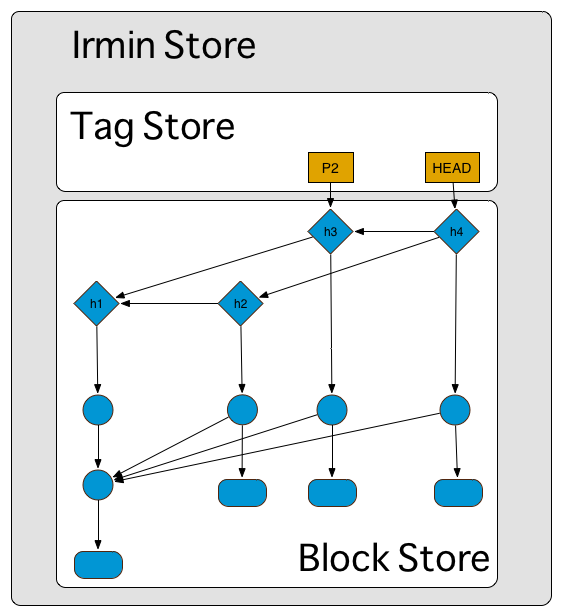
\includegraphics[width=8cm]{figs/irmin-stores.png}
			\caption{An Irmin Store composed of a mutable Tag Store and an immutable Block Store}
			\label{fig:IrminBlockStore}
			\end{center}
		\end{figure}
		For the reader familiar with Git, these can intuitively be though of as object/commits, branches and repositories respectively, however I will now explore each of these structures.
		\subsubsection*{The Block Store}
		The Irmin Block Store is a virtual heap of immutable blocks. 
		Rather than being addressed by a physical address, these blocks are addressed by the hash of their content.
		Because the block Store is content-addressable, once blocks are added, their content can never be updated.
		Instead, updates to Irmin data structures will add new blocks which try to utilise as much shared history with the existing data in the store, in order to minimise storage space.
		\subsubsection*{The Tag Store}
		Any immutability in Irmin data structures derive from tags.
		Tags provide a way of indexing into any block in the Block Store.
		This concept is similar to that of branches or references in Git, which provide a way of indexing into a particular commit in the Git history.
		Because blocks are immutable, any changes to an Irmin data structure can only be visible if a tag is updated. 
		In particular, I will refer to the HEAD tag or pointer, which will index into the latest recognised block.
		In the case of logs, this is the latest recognised log item.
		\subsubsection*{Irmin Stores}
		An Irmin Store is simply the combination of a Block Store and a Tag Store.
		Considering the criteria set out earlier for a data structure to be considered a blockchain, Irmin Stores satisfy the first criteria, i.e. that data is stored in Blocks, but not the second criteria.
		In order to satisfy these criteria, I looked to Ezirmin which provides a higher level log data structure.

	\subsection{Ezirmin}
	Ezirmin is a library that provides a simplified interface to the Irmin library. It is designed to provide a interface to Irmin without functors, but with some useful defaults. Importantly, it has a built in log data structure which uses Irmin's append-only store, saved on disk in the Git format.\\
	\begin{lstlisting}[caption={Ezirmin Log}\label{lst:ezirminlog}]
module type FS_Log = sig
  type elt 
  type cursor 
  val append : ?message:string -> branch -> path:string list -> elt -> unit Lwt.t
  val get_cursor : branch -> path:string list -> cursor option Lwt.t
  val read : cursor -> num_items:int -> (elt list * cursor option) Lwt.t
  val read_all : branch -> path:string list -> elt list Lwt.t
  ...
end
	\end{lstlisting}
	Listing \ref{lst:ezirminlog} gives some of the interface for an Ezirmin log which uses a file system backend.
	The log allows for items to be appended to and read from a log.
	In particular, the function \texttt{read} will read from the position of a cursor into the log, and will return a new cursor for the next unread log item, alongside the result.

	\subsubsection*{Ezirmin Log as a Blockchain}
	Ezirmin uses Irmin blocks as an underlying data structure, and therefore satisfies the first criteria for being considered a blockchain. 
	In order to see that the second criteria, i.e. that blocks are ordered with each containing the hash of its parent, I looked at the implementation of log items.

	\begin{lstlisting}[caption={Ezirmin Log Item}\label{lst:a_label}]
type log_item =
{ time    : Time.t;
  message : V.t;
  prev    : K.t option}
	\end{lstlisting}

	Listing \ref{lst:a_label} is taken from the Ezirmin Log implementation and shows how each log item, which is stored as a block, has a key value which points to the parent log item. 
	This imposes an ordering of log items, and means that any changes to previous log items, which will create a new block with a new address, will not be seen as part of the log. 
	As the following section details, merging logs causes new \texttt{Merge} blocks to be created with more than one log item.
	Whilst this can change the semantics of the chain of pointers between the above log items, the blockchain data structure used in this project is never merged into, so only ever contains \texttt{Value} blocks containing singular log items.
	Therefore it can be concluded that an Ezirmin Log satisfies both of my conditions to be considered a blockchain, with the definition of a 'Block' in this case being a timestamped Ezirmin log item.

	\subsubsection*{Merging Ezirmin Logs}
	Aside from using an Ezirmin Log as the blockchain data structure for this project, I also use a \textit{mempool} log to retrieve updates/transactions from remote mempools. 
	This retrieval process uses the \texttt{EzirminLog.Sync} module to merge new log items into the leader's mempool.
	In this section I will investigate the semantics of Ezirmin merges as it is critical to understanding how consensus is achieved in this project.\\
	
	Irmin allows for the developer to program custom merge strategies. 
	Whenever a synchronisation happens over the network, Irmin will do one of two things:
	\begin{enumerate}
		\item If the newly discovered blocks do not have a divergent history to the current store, they will simply be added to the block store. 
			In other words, if only new blocks have been added in the remote store, these will be added to the local store. 
		\item If the remote and local stores have divergent histories, then a custom three way merge is made using the heads of each store and their latest common ancestor.
		This merge is defined by the developer.
	\end{enumerate}
	This merge behaviour is displayed in Figure \ref{fig:ezirminmerges} where a local log performs a merge from a remote log with a diverging history.
	A custom block, \texttt{M1,2}, is created which contains both histories as defined by the custom merge function. 
	Blocks \texttt{V1} and \texttt{V2} still exist in the block store, but the HEAD tag has been updated to point to \texttt{M1,2}. \\

	Ezirmin logs make use of this functionality by storing log entries as either \texttt{Value}s or \texttt{Merge}s.
	\texttt{Value}s contain single log entries whereas \texttt{Merge}s store a list of \texttt{Values} in the order that they were created. 
	For an Ezirmin log, the custom merge takes all log entries from \texttt{Value}s and \texttt{Merge}s, orders them by their timestamps, and returns a \texttt{Merge} object with the resulting list of values. 
	This behaviour can be seen in Figure \ref{fig:ezirminmerges} by considering \texttt{Vn} to be a \texttt{Value} of the log entry \texttt{n} and \texttt{Mn,m} to be a \texttt{Merge} containing log entries \texttt{n} and \texttt{m}. 

	\begin{figure}
		\centering
		\begin{subfigure}[b]{0.40\textwidth}
			\centering
			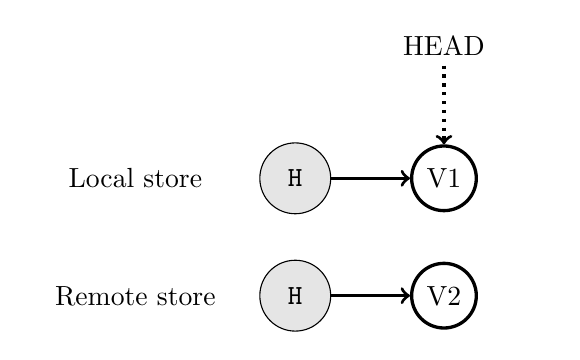
\begin{tikzpicture}[
				block/.style={circle, draw=black!100, very thick, minimum size=7mm},
				invis/.style={circle, draw=black!100, fill=black!10, minimum size=9mm},
				label/.style={rectangle, text width=2.5cm, align=center}
			]
			\node[label] (local) {Local store};
			\node[label] (remote) [below=of local] {Remote store};
			\node[invis] (gentop) [right=2mm of local]{\texttt{H}};
			\node[block] (history1) [right=of gentop] {V1};
			\node[label] (head) [above=of history1] {HEAD};
			\node[invis] (genbottom) [right=2mm of remote] {\texttt{H}};
			\node[block] (history2) [right=of genbottom] {V2};
			\begin{scope}[very thick, -stealth]
			\draw[->, dotted] (head.south) -- (history1.north);
			\draw[->] (gentop.east) -- (history1.west);
			\draw[->] (genbottom.east) -- (history2.west);
			\end{scope}
			\end{tikzpicture}
		\caption{Two Ezirmin logs diverging from a shared history, \texttt{H}.}
		\end{subfigure}
		\begin{subfigure}[b]{0.5\textwidth}
			\centering
			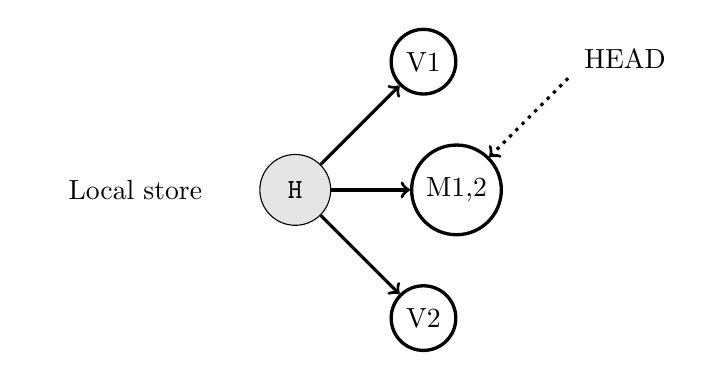
\begin{tikzpicture}[
				block/.style={circle, draw=black!100, very thick, minimum size=7mm},
				invis/.style={circle, draw=black!100, fill=black!10, minimum size=9mm},
				label/.style={rectangle, text width=2.5cm, align=center},
				labelhead/.style={rectangle, text width=1.2cm, align=center}
			]
			\node[label] (local) {Local store};
			\node[invis] (gentop)[right=2mm of local] {\texttt{H}};
			\node[block] (history1) [above right=of gentop] {V1};
			\node[block] (history2) [below right=of gentop] {V2};
			\node[block] (merge) [right=of gentop] {M1,2};
			\node[labelhead] (head) [above right=of merge] {HEAD};
			\begin{scope}[very thick, -stealth]
			\draw[->, dotted] (head.south west) -- (merge.north east);
			\draw[->] (gentop.north east) -- (history1.south west);
			\draw[->] (gentop.south east) -- (history2.north west);
			\draw[->] (gentop.east) -- (merge.west);
			\end{scope}
			\end{tikzpicture}
			\caption{After the local log has merged changes from the remote log, the HEAD tag now point to a merge item, \texttt{M1,2}, which is generated by the custom merge function.}
		\end{subfigure}
		\caption{Merging changes from a remote Ezirmin log into a local Ezirmin Log}	
		\label{fig:ezirminmerges}
	\end{figure}

	\subsubsection*{Ezirmin Bugs}
	Whilst Ezirmin provides a set of very desirable semantic properties, it is not a widely used library. 
	Consequently, during the course of the project, I encountered a couple of bugs in the Ezirmin codebase which I had to debug and fix.
	In this section I shall outline the two bugs that I encountered the changes I made to the Ezirmin codebase to fix them.\\
	
	The first bug occurs when updates are merged into a log over a network.\footnote{The issue on GitHub can be found at \href{https://github.com/kayceesrk/ezirmin/pull/7}{https://github.com/kayceesrk/ezirmin/pull/7}}
	Irmin uses Git as a backend and in order to merge updates over a network, the \texttt{git pull} command is used.
	In Git, objects are stored as blobs on the leaves of a tree and \texttt{git pull} works by retrieving all blobs at the leaf nodes of the tree for a given branch.
	However in Ezirmin, blobs can contain pointers to other blobs, which will not be retrieved by \texttt{git pull}.
	The solution that I implemented to this problem is to use an internal branch which uses an Irmin Store to add all the blobs such that they can be tracked by Git.
	Items are added to this Irmin Store on the internal banch every time they are added to the log, and consequently, this allows all log items to be fetched and merged by performing \texttt{git pull} on both the master and internal branch.\\

	The second bug that I encountered derived from the merge behaviour of Ezirmin logs when there are more than two remote machines merging updates from each others' log.\footnote{The issue on GitHub can be found at \href{https://github.com/kayceesrk/ezirmin/pull/8}{https://github.com/kayceesrk/ezirmin/pull/8}}
	The issue is that when a \texttt{Merge} block is created, it may contain log items which are stored as \texttt{Value} blocks on other machines.
	The result is that Irmin sees these blocks as different, and Ezirmin does not perform any checks to detect or remove any duplicate log items.
	This behaviour resulted from complex sequences of merge operations and so was difficult to reproduce, but in the worst case caused the size of the blockchain to grow exponentially with the number of merge operations performed.
	In one case, a log with 40 unique log items grew to be greater than 120,000 log items in size due to duplicates.
	I implemented a fix by removing duplicate log items when a merge operation takes place. 

	\section{Consensus Algorithms}
	Building consensus was by far the most important part of work completed for this project. 
	In order to guide the design of the consensus mechanism, I completed an extensive amount of research on existing algorithms
	This section will briefly summarise this research and my conclusions about their suitability for the project. 
	The resulting design for consensus is a leader based approach, where participant nodes can commit transactions to a mempool.
	This mempool is then polled for updates by the leader, and these updates are then validated and committed to the main blockchain.
	This blockchain can be read by all participants, and provides a definitive source of ordered, committed transactions.

		\subsection{Building Consensus}
			\subsubsection*{Proof of Work}
			%TODO: Use a diagram,
			Proof of Work (PoW) is a deceptively simple consensus mechanism, used by most cryptocurrencies to avoid the double spending problem.
			Transactions are contained within blocks which can be broadcast out to the network of participating nodes. 
			Whenever a block is received by a participating node, the node checks that the block contains a proof of computational work done. 
			This proof usually takes the form of a random sequence of data (this is known as a nonce) appended to the end of the block, causing the block's hash to be prefixed with a set number of 0s.
			This acts as a proof of computational work, because the data appended to the end of a block can only be found by a brute force method called mining, but can also be verified easily by simply computing the block's hash.\\
			
			Why is this useful? 
			Well, this allows us to make guarantees on the validity of the blockchain based on the simple assumption that more that 50\% of the workforce is genuine.
			If we assume that the longest chain of blocks is the correct one, then in order to create a sequence of biased transactions, we would have to create a chain longer than the correct one. 
			This would require an equal number of 'Proof of Work's, which, due to the random nature of block mining, would require more than 50\% of the workforce.
			Whilst it may be possible to maintain an equally sized chain with less that 50\% of the workforce for a short period of time, the chances of this decrease rapidly as time passes.
			All in all this means that the longer a block has been in the chain, the more likely it is that the block is valid.\\

			Whilst this forms a very effective mechanism for achieving consensus, there are also some considerable downsides to using a PoW approach to consensus. 
			Firstly, there is a huge amount of computational work wasted in the process of mining. 
			The effect of this is energy consumption \cite{BitcoinEnergy} and wastage to a level which can cause serious environmental harm.
			PoW also does not generalise well outside of the scope of cryptocurrencies.
			It assumes no trust in any participants which may not be a suitable model for an application. 
			Additionally, it also assumes that miners can be rewarded, usually with cryptocurrency, but this incentive is ad hoc and may not exist in other applications.
			
			\subsubsection*{Mempools}
			Mempools are an important part of the design of Bitcoin, and whilst they are not inherently linked to the Proof of Work consensus algorithm, they are worth investigating. 
			When a Bitcoin transaction is made, it is first written into what is known as a Mempool. 
			This transaction can then be seen by participating miners, who can then choose to put this in the next block that they mine. 
			This is significant, as it provides a 'waiting room' for any transactions that have not yet been validated.  

			\subsubsection*{Proof of Stake}
			The Proof of Stake (PoS) algorithm is used by some cryptocurrencies and works by randomly allowing participants to create (or 'forge') a single block.
			However, the probability that a participant is chosen to 'forge' a block, is weighted by its stake, such that participants with higher stakes in the blockchain are more likely to be chosen to forge a block.\\

			So, why is PoS desirable? 
			By far the most convincing reason for using PoS over PoW, is that there is no need to waste lots of energy in the process of mining. 
			This hugely reduces the environmental impacts of scaling a PoS network.
			Using PoS also allows trust to be distributed according to an arbitrary heuristic which can be desirable property in some applications.\\

			One of the flaws of PoS is that it does not have such a strong deterrent against attacks.
			With PoW, attacks require huge amounts of computational power and it is likely that to create an attack, you would have to spend more on hardware than you would gain. 
			PoS doesn't have this same built in mechanism, and so there have been many suggested schemes for increasing the safety of PoS networks.
			For example, it is possible that participants should need to pay some form of deposit before forging blocks, which can be slashed if they break any rules. 
			PoS also suffers from the same problem as PoW in that it does not generalise well. 
			It is another example of a consensus mechanism designed for networks with a strong notion of Stake and with minimal trust in any individual participant.

			\subsubsection*{Paxos}
			Paxos is a family of consensus protocols which can be used to guarantee consistency in distributed systems. 
			It was first proposed in a paper by Leslie Lamport in 1998 \cite{Paxos}, although the paper was first submitted in 1990.
			Named after a fictitious civilisation living on the island of Paxos, the algorithm puts forward a way for any number of nodes to propose and agree on a value.
			Participating nodes belong to various roles, one of which is known as a 'Proposer' or Leader.\\

			The main part of the algorithm is split into two sections, propose and accept.
			In the first stage, a Proposer decides that it wants to propose a value and then broadcasts out a 'Prepare' message to a quorum of 'Acceptors'.
			Acceptors will then decide if they want to make a 'Promise' which is a commitment to accepting that proposal in the future. 
			If a quorum of promises is received by the Proposer, then it will assign a value to its proposal and will again send an 'Accept Request' out to a quorum of Acceptors.
			Finally, if enough 'Accept' messages are received then the Proposer can be certain that the value has been agreed upon by consensus.\\

			This algorithm has been proved to be consistent but it also has a lot of complexity and a lot of different variants. 
			The combination of different roles and states makes it easy to implement incorrectly.
			It is also important to consider that Paxos describes a 'family' of algorithms, with some parts left deliberately unspecified, and choosing how to implement these is not a trivial decision.
			The final issue with Paxos is that it cannot guarantee progress.
			Whilst it enforces conditions which make it unlikely that progress will not be made, it is still theoretically possible for the mechanism to stall indefinitely.

			\subsubsection*{Raft}
			Raft \cite{Raft} is an algorithm that was designed to be equivalent and as efficient as Paxos, however, it also places a much greater emphasis on comprehensibility.
			It uses the notion of a \textit{strong leader}, which is an elected server that has total control over which log entries are accepted.
			There are two other types of server, a \textit{follower} and a \textit{candidate}. 
			Followers are completely passive, and only respond to requests from leaders and candidates. 
			A candidate is a server that has put itself forward for election.\\

			So how does the algorithm operate? 
			Time in Raft is split into \textit{terms} which are labelled by a monotomically increasing integer. 
			Each term effectively signals a time period where a particular server is the leader. 
			A term starts with a leadership election when a follower transitions into the candidate state, increments its term number and requests votes from other servers. 
			It will wait for a majority of votes and then elect itself the leader, unless it times out or receives a message from another leader with a greater term number. 
			Typically, these leader election processes are triggered when a follower doesn't receive a heartbeat message from the leader for longer than a given time.
			In the pathological case, the vote can be split between leaders, triggering a new election which is also split and so on.
			However, Raft uses randomised election timeouts to avoid this problem.
			Additionally, Raft also prescribes some restrictions on the servers which can be elected leader so as to avoid newly elected leaders overwriting previously appended log items.\\
			
			Raft is an simple algorithm that is easy to understand, but it also guarantees the Log Matching Property that if two logs contain a log entry with the same index and term, then that entry, and all preceding entries will be identical.

		\subsection{A New Approach}
		I have build a consensus mechanism that uses a mempool and a simple leader based algorithm. 
		Because I have implemented a centralised algorithm, my specification has differed slightly from that presented in the \nameref{Requirements Analysis} to take into account differing functional requirements for a leader and for a participant.
		As I am assuming that all participating nodes can be trusted, it is possible to use a leader based approach without introducing security issues such as the ones tackled by the Proof of Work mechanism. 
		This approach also reduces the potential complexity of implementing completely decentralised consensus.
		My approach makes use of the mergeable log data structure provided by Ezirmin, and the synchronisation module that allows updates from a log to be pulled into another.
		Finally, I have introduced the notion of validation which allows both participants and leader nodes to accept or reject transactions depending on arbitrary conditions.
		
			\subsubsection*{Leaders}
			My consensus mechanism uses the notion of a \textit{strong leader} similar to that used by the Raft protocol. 
			The leader is chosen statically in order to reduce the complexity of implementation, and it also has a statically defined list of \texttt{remotes} which specifies the location of all participants.
			The leader is a node which will never actually request transactions to be added to the blockchain, its role is simply to periodically read requests from the mempools of participants, validate them, and then add them to the blockchain.
			This blockchain can be read by any participant, and is treated as the empirical source of which transactions have been committed and in which order. 
			That is, any two nodes that read a copy of the blockchain, will always agree on content and ordering of log items in the blockchain, up until the end of the shortest copy (or both copies).\\

			\begin{lstlisting}[caption={Leader Specification}\label{lst:leaderspec}]
module type I_LeaderConfig = sig
  type t
  module LogCoder: Participant.I_LogStringCoder with type t = t    
  val remotes: string list
  val validator: (t list -> t list -> t list) option
end
module type I_Leader = sig
  val init_leader: unit -> (unit -> unit Lwt.t) Lwt.t
end
module MakeLeader (Config: I_LeaderConfig) : I_Leader = struct
  ...
end
			\end{lstlisting}

			Listing \ref{lst:leaderspec} is the specification of the leader module, which differs slightly from the centralised specification presented in the \nameref{Requirements Analysis}.
			In particular, the \texttt{init\_leader} function will perform an initialisation step, and then return a function which, when executed, will actually start the consensus process.

			\subsubsection*{Participants}
			Participants, in contrast to leaders, can request transactions to be added to the blockchain. 
			This is done by writing a transaction to a local mempool, which is then read by the leader.
			Validation can of this transaction can also happen at this stage, but as we'll see later, it cannot filter out all invalid transactions, and only exists to ease load on the leader.\\

			\begin{lstlisting}[caption={Participant Specification}\label{lst:partspec}]
module type I_LogStringCoder = sig
  type t
  val encode_string: t -> string
  val decode_string: string -> t option
end
module type I_ParticipantConfig = sig
  type t
  module LogCoder: I_LogStringCoder with type t = t
  val leader_uri: string option
  val validator: (t list -> t -> bool) option
end
module type I_Participant = sig
  type t
  val add_transaction_to_mempool: t -> [> `Could_Not_Pull_From_Remote | `Validation_Failure | `Ok] Lwt.t
  val get_transactions_from_blockchain: int -> [> `Error | `Ok of t list] Lwt.t
  val get_all_transactions_from_blockchain: unit -> [> `Error | `Ok of t list] Lwt.t
end
module Make(Config: I_ParticipantConfig): I_Participant with type t = Config.t = struct
  ...
end
			\end{lstlisting}

			Listing \ref{lst:partspec} is a specification that shines a light on the role of participants and the functionality they provide.
			The module includes the ability to define custom data types that can be stored on the blockchain, to define how to validate transactions, to read from the blockchain, and to attempt to write to the blockchain by writing to a mempool.

			\subsubsection*{Retrieving local updates}
			The mechanism used by the leader to read mempool updates is different for the situations when the participant is on the same machine, and when it is on a remote machine. 
			Here, I will detail the process of reading updates from a participant on the same machine as the leader.\\

			\begin{figure}
				\begin{center}
					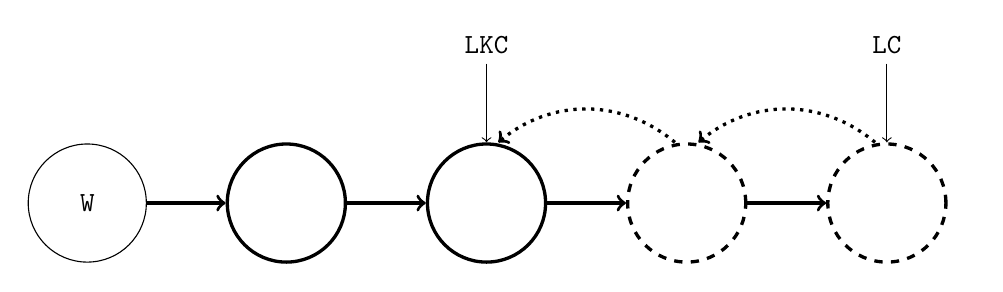
\begin{tikzpicture}[
						block/.style={circle, draw=black!100, very thick, minimum size=15mm},
						invis/.style={circle, draw=black!100, minimum size=15mm},
						label/.style={rectangle, text width=2cm, align=center}
					]
					\node[invis] (invis) {\texttt{W}};
					\node[block] (block1) [right=of invis] {};
					\node[block] (block2) [right=of block1] {};
					\node[label] (label1) [above=of block2] {\texttt{LKC}};
					\node[block] (block3) [right=of block2, dashed] {};
					\node[block] (block4) [right=of block3, dashed] {};
					\node[label] (label2) [above=of block4] {\texttt{LC}};
					\draw[->] (label2.south) -- (block4.north);
					\draw[->] (label1.south) -- (block2.north);
					\begin{scope}[very thick, -stealth]
					\draw[->] (invis.east) -- (block1.west);
					\draw[->] (block1.east) -- (block2.west);
					\draw[->] (block2.east) -- (block3.west);
					\draw[->] (block3.east) -- (block4.west);
					\path[dotted, ->] (block4.north)+(-1.5mm,0) edge  [bend right=40]  ([xshift=1.5mm]block3.north);
					\path[dotted, ->] (block3.north)+(-1.5mm,0) edge  [bend right=40]  ([xshift=1.5mm]block2.north);
					\end{scope}
					\end{tikzpicture}
					\end{center}
				\caption{A mempool on a local participant. \texttt{W} indicates the history of a \textit{Worker's} mempool. Blocks with dashed outlines represent transactions that have not yet been added to the blockchain. \texttt{LKC} and \texttt{LC} are the \textit{Latest Known Cursor} and the \textit{Latest Cursor} respectively.}
				\label{fig:readlocalpartudpates}
			\end{figure}

			The leader will always maintain a cursor to the latest entry it has read from the participant mempool.
			When it attempts to find new updates, it will get a new cursor to the latest element of the mempool.
			The leader can then compare these two cursors, and if the \textit{latest known} cursor points to an entry with an earlier timestamp than the \textit{latest} cursor, then it will add the \textit{latest} item to an accumulator, and then repeat the process with a cursor pointing to the parent of the \textit{latest} node. 
			Finally, when the cursors match, the items in the accumulator are returned as new updates which can be added to the leader mempool and the \textit{latest known} cursor is updated accordingly.
			It is important to note that no validation is performed at this stage as no item has been added to the blockchain yet.
			Figure \ref{fig:readlocalpartudpates} shows how unseen blocks are read sequentially from a mempool until the seen blocks are reached.
	
			\subsubsection*{Retrieving remote updates}
			The previous section demonstrates how updates can be retrieved from a mempool on the same machine as the leader.
			In this section, I will highlight how updates are retrieved from mempools on remote machines.\\
			
			Irmin provides a \texttt{Sync} module which allows for the histories of a local and a remote Store to be combined according to a custom merge function.
			Ezirmin logs build on this functionality by providing a merge strategy which uses the log entry timestamps to order log entries in a merge.
			Figure \ref{fig:readremotepartudpates} demonstrates how this merge works in a situation where a number of blocks have been added to a single remote participant mempool.
			The first (and most na{\"i}ve) approach I took to pulling updates from a number of participants, was to sequentially merge updates from all the participants into the leaders mempool.
			Participants also merge updates from the leader's mempool before adding to their own mempool to increase the shared history and decrease the work required for the leader to perform the merge.
			After pulling all updates, the leader will traverse its own mempool, finding new updates until it reaches the \textit{latest known} cursor. 
			Now, the updates can be validated and added to the blockchain, and the \textit{latest known} cursor updated to the latest message in the mempool.\\

			\begin{figure}
				\centering
				\begin{subfigure}[b]{0.45\textwidth}
					\centering
					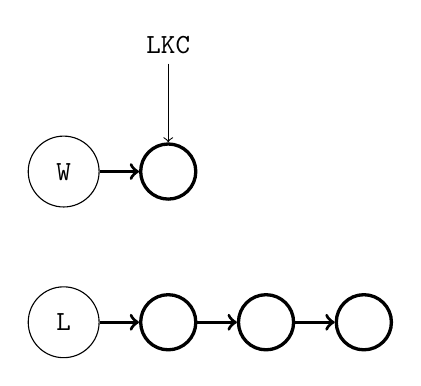
\begin{tikzpicture}[
						block/.style={circle, draw=black!100, very thick, minimum size=7mm},
						invis/.style={circle, draw=black!100, minimum size=9mm},
						label/.style={rectangle, text width=1.2cm, align=center}
					]
					\node[invis] (invis1) {\texttt{L}};
					\node[invis] (invis2) [above=of invis1] {\texttt{W}};
					\node[block] (n) [right=5mm of invis1] {};
					\node[block] (m) [right=5mm of invis2] {};
					\node[block] (n1) [right=5mm of n] {};
					\node[block] (n2) [right=5mm of n1] {};
					\node[label] (latest) [above=of m] {\texttt{LKC}};
					\draw[->] (latest.south) -- (m.north);
					\begin{scope}[very thick, -stealth]
					\draw[->] (invis1.east) -- (n.west);
					\draw[->] (invis2.east) -- (m.west);
					\draw[->] (n.east) -- (n1.west);
					\draw[->] (n1.east) -- (n2.west);
					\end{scope}
					\end{tikzpicture}
				\caption{Before merge}
				\end{subfigure}
				\begin{subfigure}[b]{0.45\textwidth}
					\centering
					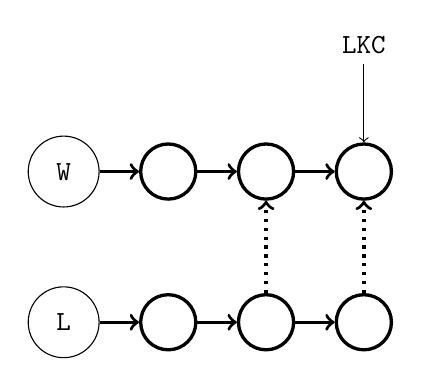
\begin{tikzpicture}[
						block/.style={circle, draw=black!100, very thick, minimum size=7mm},
						invis/.style={circle, draw=black!100, minimum size=9mm},
						label/.style={rectangle, align=center, text width=1.2cm}
					]
					\node[invis] (invis1) {\texttt{L}};
					\node[invis] (invis2) [above=of invis1] {\texttt{W}};
					\node[block] (n) [right=5mm of invis1] {};
					\node[block] (m) [right=5mm of invis2] {};
					\node[block] (m1) [right=5mm of m] {};
					\node[block] (m2) [right=5mm of m1] {};
					\node[block] (n1) [right=5mm of n] {};
					\node[block] (n2) [right=5mm of n1] {};
					\node[label] (latest) [above=of m2] {\texttt{LKC}};
					\draw[->] (latest.south) -- (m2.north);
					\begin{scope}[very thick, -stealth]
					\draw[->] (invis1.east) -- (n.west); 
					\draw[->] (m.east) -- (m1.west);
					\draw[->] (m1.east) -- (m2.west);
					\draw[dotted,->] (n1.north) -- (m1.south);
					\draw[dotted,->] (n2.north) -- (m2.south);
					\draw[->] (invis2.east) -- (m.west);
					\draw[->] (n.east) -- (n1.west);
					\draw[->] (n1.east) -- (n2.west);
					\end{scope}
					\end{tikzpicture}
				\caption{After merge}
				\end{subfigure}
				\caption{Merging mempool updates and adding to the blockchain from a single remote participant (below) to leader (above). \texttt{W} and \texttt{L} respectively signify the histories of the \textit{Worker's} and \textit{Leader's} mempools.}	
				\label{fig:readremotepartudpates}
			\end{figure}

			However, this approach is fundamentally flawed and causes many updates to be overlooked by the leader. 
			This is because of the delays that occur when mempool updates are retrieved over the network from multiple workers.
			For example, Figure \ref{fig:readremotepartudpatesbroke} demonstrates a situation where there are just two workers. 
			In this case, updates from the first worker will be merged before the second, however, after the first merge has taken place, the first worker may have added additional transactions. 
			If these transactions are timestamped before the latest transaction in the second worker's mempool, then when the leader next polls for updates, transactions may be merged to a position in the mempool before the latest known cursor. 
			This means that they will not be seen by the leader and therefore they will not be added to the blockchain. 
			I shall refer to these transactions as \textit{missed} transactions, and all others at \textit{tracked} transactions.\\

			\begin{figure}
				\centering
				\begin{subfigure}[b]{0.45\textwidth}
					\centering
					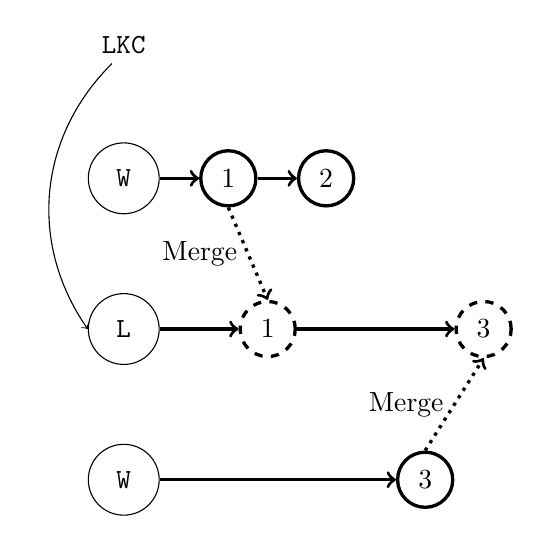
\begin{tikzpicture}[
						block/.style={circle, draw=black!100, very thick, minimum size=7mm},
						invis/.style={circle, draw=black!100, minimum size=9mm},
						label/.style={rectangle, text width=1.2cm, align=center}
					]
					\node[invis] (gentop) {\texttt{W}};
					\node[invis] (genmiddle) [below=of gentop] {\texttt{L}};
					\node[invis] (genbottom) [below=of genmiddle] {\texttt{W}};
					\node[block] (one) [right=5mm of gentop] {1};
					\node[block] (onemerged) [right=10mm of genmiddle, dashed] {1};
					\node[block] (two) [right=5mm of one] {2};
					\node[block] (three) [right=30mm of genbottom] {3};
					\node[block] (threemerged) [right=20mm of onemerged, dashed] {3};
					\node[label] (latestknown) [above=of gentop] {\texttt{LKC}};
					\path[->] (latestknown.south)+(-1.5mm,0) edge  [bend right=40]  (genmiddle.west);
					\begin{scope}[very thick, -stealth]
					\draw[->] (gentop.east) -- (one.west);
					\draw[dotted, ->] (one.south) -- (onemerged.north) node[midway, left] {Merge};
					\draw[dotted, ->] (three.north) -- (threemerged.south) node[midway, left] {Merge};
					\draw[->] (onemerged.east) -- (threemerged.west);
					\draw[->] (one.east) -- (two.west);
					\draw[->] (genmiddle.east) -- (onemerged.west);
					\draw[->] (genbottom.east) -- (three.west);
					\end{scope}
					\end{tikzpicture}
				\caption{After first sync from leader. Transactions 1 and 3 are merged after the latest known transaction and are therefore \textit{tracked}}
				\end{subfigure}
				\begin{subfigure}[b]{0.45\textwidth}
					\centering
					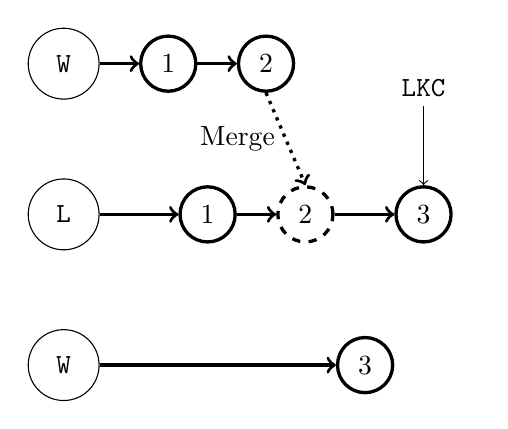
\begin{tikzpicture}[
						block/.style={circle, draw=black!100, very thick, minimum size=7mm},
						invis/.style={circle, draw=black!100, minimum size=9mm},
						label/.style={rectangle, text width=1.2cm, align=center}
					]
					\node[invis] (gentop) {\texttt{W}};
					\node[invis] (genmiddle) [below=of gentop] {\texttt{L}};
					\node[invis] (genbottom) [below=of genmiddle] {\texttt{W}};
					\node[block] (one) [right=5mm of gentop] {1};
					\node[block] (onemerged) [right=10mm of genmiddle] {1};
					\node[block] (two) [right=5mm of one] {2};
					\node[block] (twomerged) [right=5mm of onemerged, dashed] {2};
					\node[block] (three) [right=30mm of genbottom] {3};
					\node[block] (threemerged) [right=20mm of onemerged] {3};
					\node[label] (latestknown) [above=of threemerged] {\texttt{LKC}};
					\draw[->] (latestknown.south) -- (threemerged.north);
					\begin{scope}[very thick, -stealth]
					\draw[->] (gentop.east) -- (one.west);
					\draw[dotted, ->] (two.south) -- (twomerged.north) node[midway, left] {Merge};
					\draw[->] (onemerged.east) -- (twomerged.west);
					\draw[->] (twomerged.east) -- (threemerged.west);
					\draw[->] (one.east) -- (two.west);
					\draw[->] (genmiddle.east) -- (onemerged.west);
					\draw[->] (genbottom.east) -- (three.west);
					\end{scope}
					\end{tikzpicture}
					\caption{After second round of leader synchronisation, transaction 2 is merged into the mempool before the latest known transaction and is therefore \textit{missed}}
				\end{subfigure}
				\caption{In this diagram, time flows from left to right. 
				The sequential nature of mempool merges causes transaction 2 to be merged into the history of the mempool before the transaction pointed to by the latest known cursor. 
				2 will therefore not be added to the blockchain.}	
				\label{fig:readremotepartudpatesbroke}
			\end{figure}

			In order to mitigate this problem, I first examined the nature of these \textit{missed} transactions and noted the following properties:
			\begin{enumerate}
				\item Missed transactions must have been added during a merge. If they occured before the merge had begun, then they would have been tracked. 
				Alternatively, missed transactions must occur after the latest known cursor from the previous merge. 
				\item Missed transactions must have been added at a point in time earlier than the transaction pointed to by the latest\_known cursor. 
				If they occured at a later point in time, then they would be tracked by future leader polls.
			\end{enumerate}

			These lead very naturally onto a less na{\"i}ve algorithm for retrieving updates which only adds updates that have existed for more than one 'poll cycle'.
			Instead of maintaining a single cursor to the latest-known item, another cursor is now maintained to the previous latest-known item. 
			I will refer to these as the \texttt{latest\_known} and \texttt{previous\_latest\_known} items.
			After merging the newest set of updates, a leader can be sure that no more missed transactions will be added before the \texttt{latest\_known} item, and after the \texttt{previous\_latest\_known} item. 
			\begin{lstlisting}[caption={Selecting new updates}\label{lst:newupdates}]
let is_early_enough = is_earlier_or_equal scanning_cursor ~than:latest_known in
let is_late_enough = is_later scanning_cursor ~than:previous_latest_known in
match is_early_enough, is_late_enough with
  | Some(false), Some(true) -> (*Item cannot be added to blockchain yet. Move scanning cursor back by one item and loop*)
  | Some(true), Some(true) -> (*Item can be added to blockchain. Add item to accumulator, move cursor back by one item and loop*)
  | _ ->(*Too far back in the mempool, so return item accumulator*)
			\end{lstlisting}

			Listing \ref{lst:newupdates} shows a snippet of code from within a recursive function to get updates from the mempool, which can be added to the blockchain.
			This demonstrates a new approach which starts with a newly retrieved cursor, \texttt{scanning\_cursor}, to the latest mempool element and then scans back through the mempool, adding valid items to an accumulator and eventually returning.
			On each loop, this algorithm will check if the item is valid, adding the item to the accumulator if this is the case, and then either return the accumulator or move the \texttt{scanning\_cursor} to the next item back in the mempool.
			Every item from the \texttt{latest\_known} item (inclusive) to the \texttt{previous\_latest\_known} item (exclusive) will be added to the blockchain. 
			Any of the further updates are not safe to add, and will be postponed until the next poll.
			In the case that both cursors point to the same item (i.e. no new items were retrieved in the latest poll), no items are added as it is always assumed that the \texttt{latest\_known} item is added in the previous poll.
			The cursors can now be updated as follows, where \texttt{get\_new\_latest\_cursor} will get a cursor to the latest item in the leader's mempool.
			\begin{lstlisting}
previous_latest_known_cursor := latest_known_cursor;;
latest_known_cursor := get_new_latest_cursor;;
			\end{lstlisting}
			
			This approach will not only pick up all the previously missed transactions, but all the tracked ones too.
			Figure \ref{fig:readremotepartudpatesfixed} demonstrates how this approach would solve the problem presented in Figure \ref{fig:readremotepartudpatesbroke}.\\

			\begin{figure}
			\centering
			\begin{subfigure}[b]{0.45\textwidth}
				\centering
				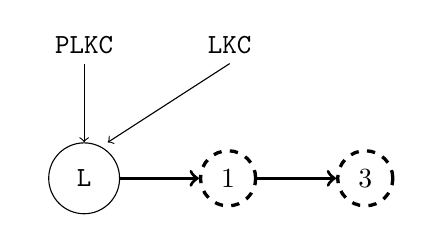
\begin{tikzpicture}[
					block/.style={circle, draw=black!100, very thick, minimum size=7mm},
					invis/.style={circle, draw=black!100, minimum size=9mm},
					label/.style={rectangle, text width=1.2cm, align=center}
				]
				\node[invis] (genmiddle) {\texttt{L}};
				\node[block] (onemerged) [right=10mm of genmiddle, dashed] {1};
				\node[block] (threemerged) [right=of onemerged, dashed] {3};
				\node[label] (prevlatestknown) [above=of genmiddle] {\texttt{PLKC}};
				\node[label] (latestknown) [right=4mm of prevlatestknown] {\texttt{LKC}};
				\draw[->] (latestknown.south) -- ([xshift=3mm] genmiddle.north);
				\draw[->] (prevlatestknown.south) -- (genmiddle.north);
				\begin{scope}[very thick, -stealth]
				\draw[->] (onemerged.east) -- (threemerged.west);
				\draw[->] (genmiddle.east) -- (onemerged.west);
				\end{scope}
				\end{tikzpicture}
			\caption{After first merge, items 1 and 3 have been merged but not added to the blockchain.}
			\end{subfigure}
			\begin{subfigure}[b]{0.45\textwidth}
				\centering
				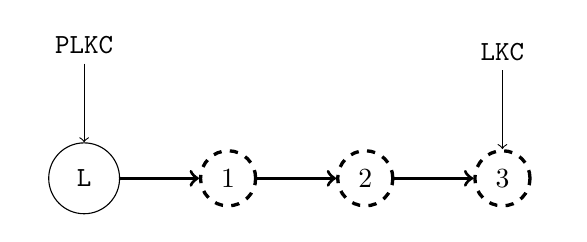
\begin{tikzpicture}[
					block/.style={circle, draw=black!100, very thick, minimum size=7mm},
					invis/.style={circle, draw=black!100, minimum size=9mm},
					label/.style={rectangle, text width=1.2cm, align=center}
				]
				\node[invis] (genmiddle) {\texttt{L}};
				\node[block] (onemerged) [right= of genmiddle, dashed] {1};
				\node[block] (twomerged) [right= of onemerged, dashed] {2};
				\node[block] (threemerged) [right= of twomerged, dashed] {3};
				\node[label] (prevlatestknown) [above=of genmiddle] {\texttt{PLKC}};
				\node[label] (latestknown) [above=of threemerged] {\texttt{LKC}};
				\draw[->] (prevlatestknown.south) -- (genmiddle.north);
				\draw[->] (latestknown.south) -- (threemerged.north);
				\begin{scope}[very thick, -stealth]
				\draw[->] (onemerged.east) -- (twomerged.west);
				\draw[->] (twomerged.east) -- (threemerged.west);
				\draw[->] (genmiddle.east) -- (onemerged.west);
				\end{scope}
				\end{tikzpicture}
				\caption{After second merge, item 2 is now part of the mempool history, and items 1, 2, and 3 can be added to the blockchain.}
			\end{subfigure}
			\begin{subfigure}[b]{0.45\textwidth}
				\centering
				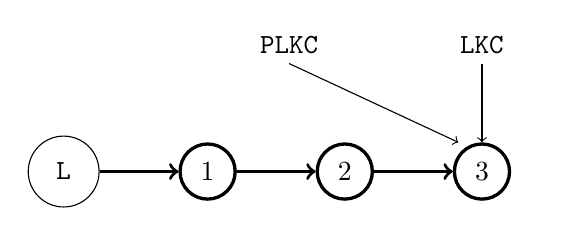
\begin{tikzpicture}[
					block/.style={circle, draw=black!100, very thick, minimum size=7mm},
					invis/.style={circle, draw=black!100, minimum size=9mm},
					label/.style={rectangle, text width=1.2cm, align=center}
				]
				\node[invis] (genmiddle) {\texttt{L}};
				\node[block] (onemerged) [right= of genmiddle] {1};
				\node[block] (twomerged) [right= of onemerged] {2};
				\node[block] (threemerged) [right= of twomerged] {3};
				\node[label] (latestknown) [above=of threemerged] {\texttt{LKC}};
				\node[label] (prevlatestknown) [left=of latestknown] {\texttt{PLKC}};
				\draw[->] (prevlatestknown.south) -- ([xshift=-3mm]threemerged.north);
				\draw[->] (latestknown.south) -- (threemerged.north);
				\begin{scope}[very thick, -stealth]
				\draw[->] (onemerged.east) -- (twomerged.west);
				\draw[->] (twomerged.east) -- (threemerged.west);
				\draw[->] (genmiddle.east) -- (onemerged.west);
				\end{scope}
				\end{tikzpicture}
				\caption{After second merge, items 1, 2 and 3 have been added to the blockchain.}
			\end{subfigure}
			\caption{Using two cursors, any missed items can be caught and added to the blockchain. \texttt{PLKC} signifies the \textit{Previous Latest Known Cursor}.}	
			\label{fig:readremotepartudpatesfixed}
		\end{figure}

		At a first glance, it may seem sensible to use the \texttt{latest\_known} cursor to get new updates from the mempool by just iterating back through the mempool from cursor.
		The problem with this approach is that the cursor is an abstraction of a tag to a block in the Irmin Block Store.
		This means that the history of the mempool according to that cursor is not changed by any subsequent merge operations.
		Consequently, any \textit{missed} transactions will not be visible using this approach.\\

		This now begs the question 'How can the new approach, which uses out-of-date cursors, still be valid?'.
		The answer to this is that, the new approach only uses the cursors to perform timestamp comparisons.
		The result of these comparisons is the same whether a cursor to the items in the out-of-date mempool or a cursor to the items in the new mempool is used.

	\chapter{Evaluation}
	
	\chapter{Conclusion}
	
	
	%%%%%%%%%%%%%%%%%%%%%%%%%%%%%%%%%%%%%%%%%%%%%%%%%%%%%%%%%%%%%%%%%%%%%
	% the bibliography
	\bibliographystyle{acm}
	\bibliography{refs}
	\addcontentsline{toc}{chapter}{Bibliography}
	
	%%%%%%%%%%%%%%%%%%%%%%%%%%%%%%%%%%%%%%%%%%%%%%%%%%%%%%%%%%%%%%%%%%%%%
	% the appendices
	\appendix

	\chapter{Project Proposal}
	
	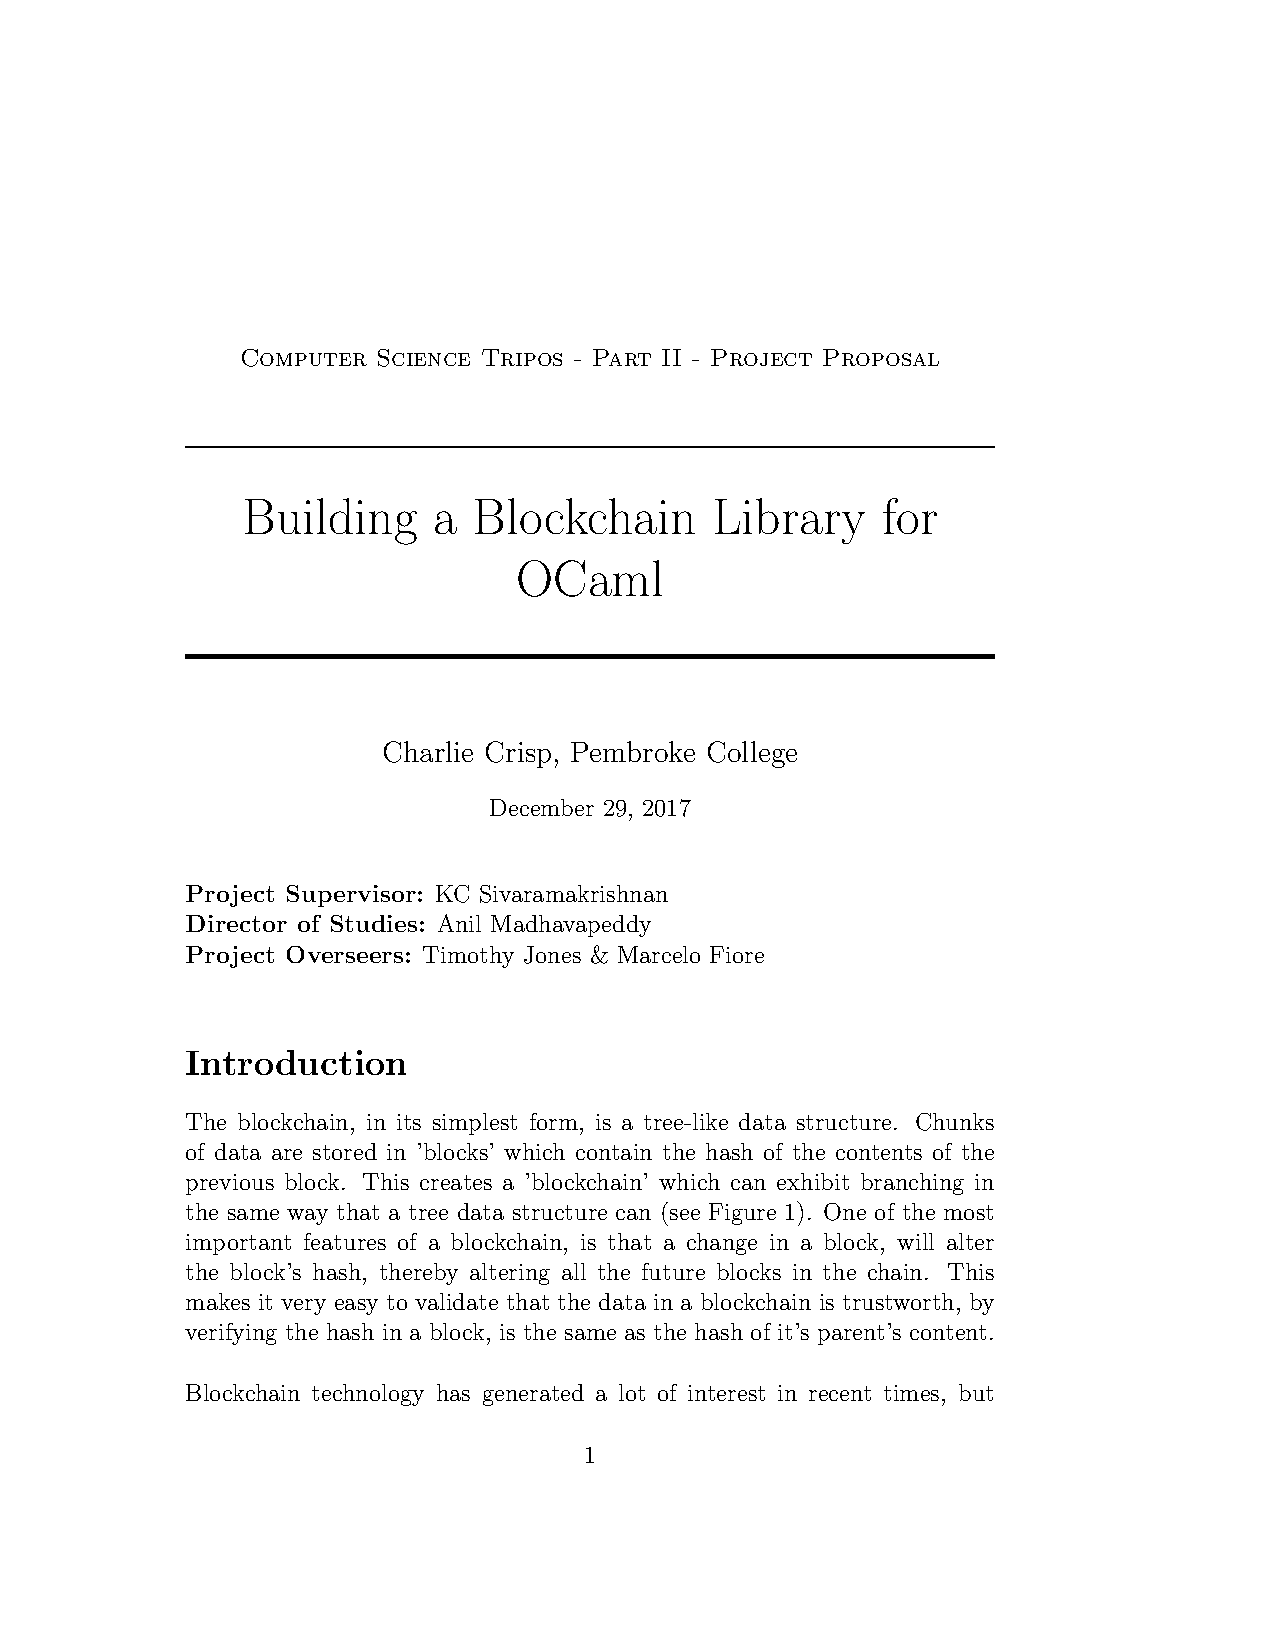
\includepdf[pages=-]{Part_II_Project_Proposal_Draft.pdf}
	
	\end{document}